\documentclass[11pt,a4paper,english,oneside, pdf]{article}
\usepackage[margin=2.5cm]{geometry}
\usepackage[utf8]{inputenc} %Permite introducir directamente acentos: á en lugar de \'a etc.
\usepackage{mathtools}
\usepackage{palatino}
\usepackage{graphicx}
\usepackage{hyperref}
\usepackage{xcolor}

\title{BACoN analysis RUN 3}
\author{Carmen Romo Luque}

\graphicspath{{/Users/romoluque_c/Repositories/BACON_romo/analysis_documentation/images/}}

\begin{document}
	\maketitle
	
	\section{Introduction}	 
	 The BACoN detector is designed to investigate the scintillation properties of liquid argon when doped with xenon. The setup consists of a 100-liter cylindrical cryostat filled with liquid argon, featuring a single upward-facing PMT mounted at the bottom and four rows of three equidistantly spaced SiPMs. Each SiPM row is separated by 10 cm from the next one. On top of the cylinder, an Americium source is placed, emitting gammas and alphas that interact with the liquid, producing scintillation light. The first row of SiPMs is positioned close to the decay source and serves as the trigger system when all of them detect at least one photoelectron. These three SiPMs are collimated to prevent potential saturation effects.
	 
	 %\begin{figure}[!h]
	 %	\begin{center}
	 %		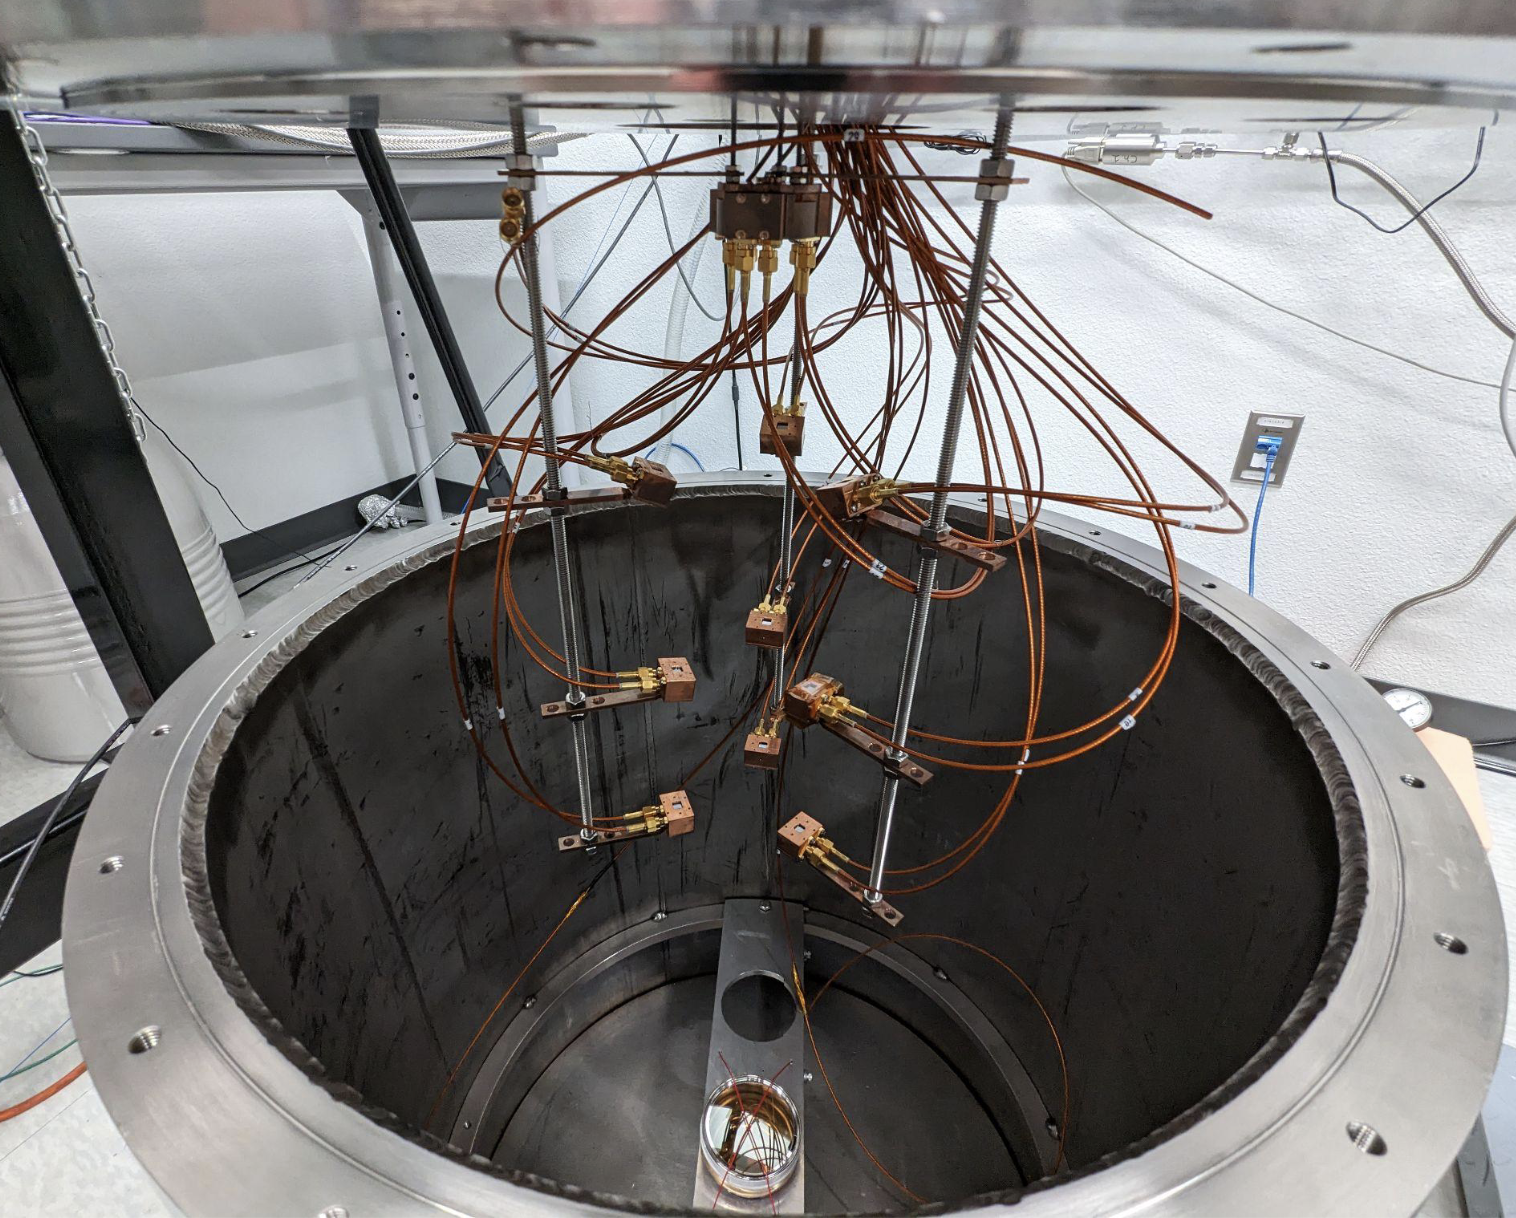
\includegraphics[width=9cm]{BACoN_picture_run2}
	 %		\caption{New setup of the BACoN detector. The PMT is placed at the bottom of the chamber and 4 rows of SiPMs arranged around 10 cm apart, facing the americium source.}
	 %		\label{fig:BACoN_picture_run2}
	 %	\end{center}
	 %\end{figure}
	 
	 The cryostat's liquid argon level is continuously monitored by measuring its weight. Additionally, the argon undergoes purification via a SAES PS4-MT3/15-R getter, which removes impurities such as H$_2$0, CO, CO$_2$, N$_2$, H$_2$, CH$_4$, reducing their concentrations to less than 1 part per billion (PPB) prior to liquefaction.
	 
	 
	 \clearpage
	
	\section{SiPM calibration}
	\label{cal_dark_box}
	
	Maintaining the optimal performance of sensors in the BACoN system is crucial for accurate data collection, enabling the detection of variations in light levels within the detector. For this, periodic calibrations of the SiPMs are conducted to verify their proper functioning and stability. Despite employing the same sensor model across all SiPMs, variations in analog-to-digital conversion (ADC) counts in response to identical light inputs are inevitable. Hence, regular calibration of the SiPMs at the single photon level is imperative to standardize their responses and assess their long-term stability.
	
	Ideally, a chamber should be equipped with LEDs for performing regular calibrations during data collection. That would allow us to monitor gain variations over time at a controlled light intensity, particularly important for long-term data acquisitions lasting several months or few years. Additionally, since we operate at low temperatures, the gains of the SiPMs won't match those obtained during black box calibration. However, in the absence of LEDs, we can still utilize low-light data for similar calibrations, though it's important to note that the values may differ.
	
	Due to the low temperature required to maintain argon in its liquid state within the BACoN detector, the bias voltage of the SiPMs needs to be reduced. This compensates for the decrease in breakdown voltage of the silicon diodes within the SiPM structure under reduced thermal conditions. At lower temperatures, the breakdown voltage tends to increase, meaning that the same bias voltage applied at room temperature could potentially cause the SiPMs to operate in a regime where the breakdown voltage is exceeded. This can lead to excess dark count rate and decreased performance. Therefore, reducing the bias voltage when operating SiPMs at lower temperatures helps ensure that they remain within their optimal operating conditions and maintain stable performance. That's the reason why the gains of the SiPMs inside the chamber are higher even at a lower bias voltage.
		

	
	First, we subtract the baseline of the waveform, which allows us to obtain the absolute height of the peaks. The baseline subtraction procedure can be performed by computing either the mean value or the mode of the entire waveform or just a certain range. 
	Then, we compute the single photon spectra by getting the height of the peaks at the trigger region. 

	
	Subsequently, a histogram is generated displaying the heights of the peaks in the trigger window, allowing for the identification of individual single photoelectron peaks. First, a poisson distribution of a certain number of gaussians is perfomed in order to extract the mean position of each photoelectron peak. The gain is then calculated from the spectrum using the distance between the pedestal peak and those for 1, 2, ...  photoelectrons.
	
	
	Then, the linear regression of the mean achieved enables the extraction of the conversion factor between ADC and photoelectrons. With these values, the response across all channels can be standardize.
	
	
	
	
	\subsection{Baseline}
	
	
	The first check of the 12 SiPMs and the PMT data is the baseline. The baseline can be computed used the mean or the mode of a selected range of the waveform. Since the trigger time in BACoN is close to 1500 ns, to havoid having peaks in the chosen region, we use the first 1000 ns of the waveform. Figure \ref{fig:baselines} shows the baseline over time for some runs taken in September. The baseline seems to be decreasing over time and the deviation from the mean is higher in the trigger SiPMs than in the normal SiPMs.
	
	\begin{figure}[!h]
		\begin{center}
			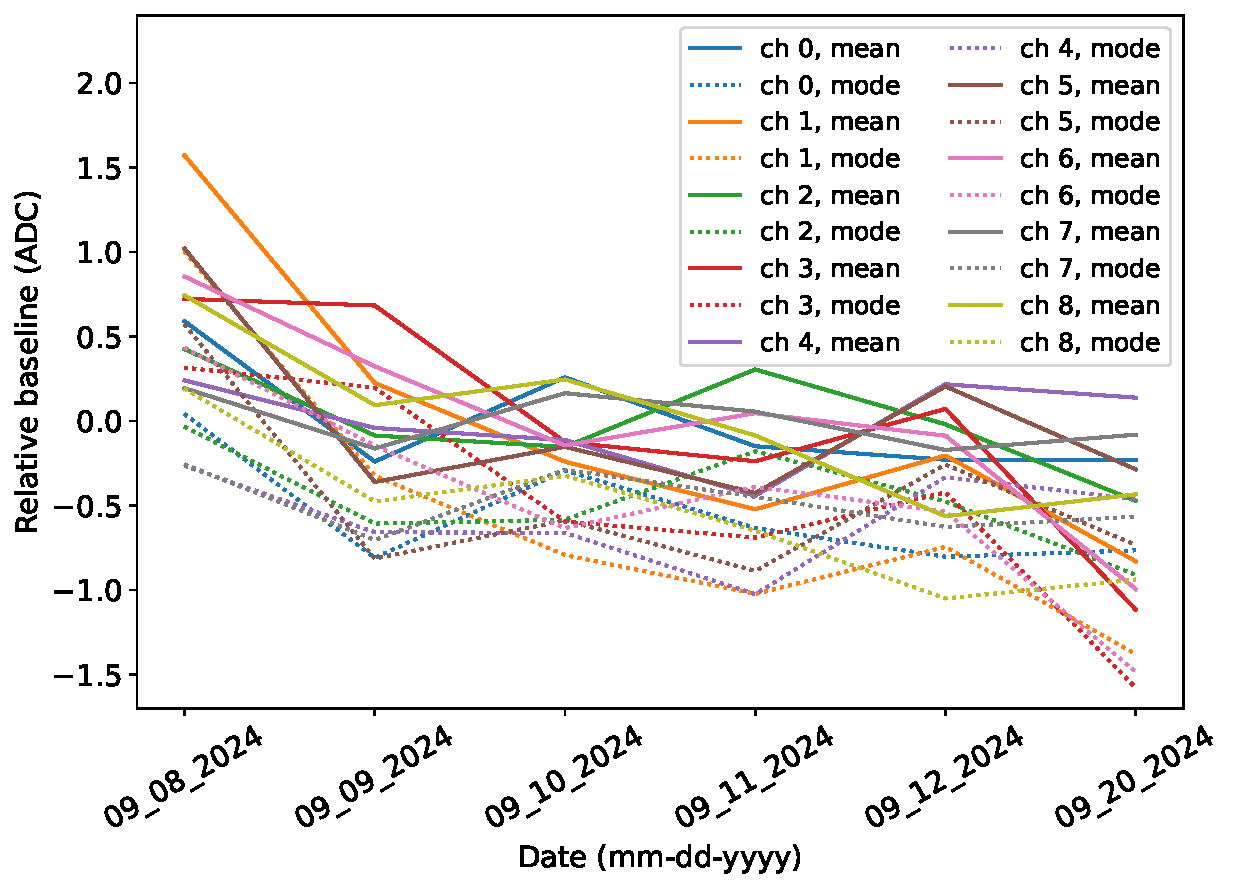
\includegraphics[width=0.49\textwidth]{images/baselines_rel1.pdf}
			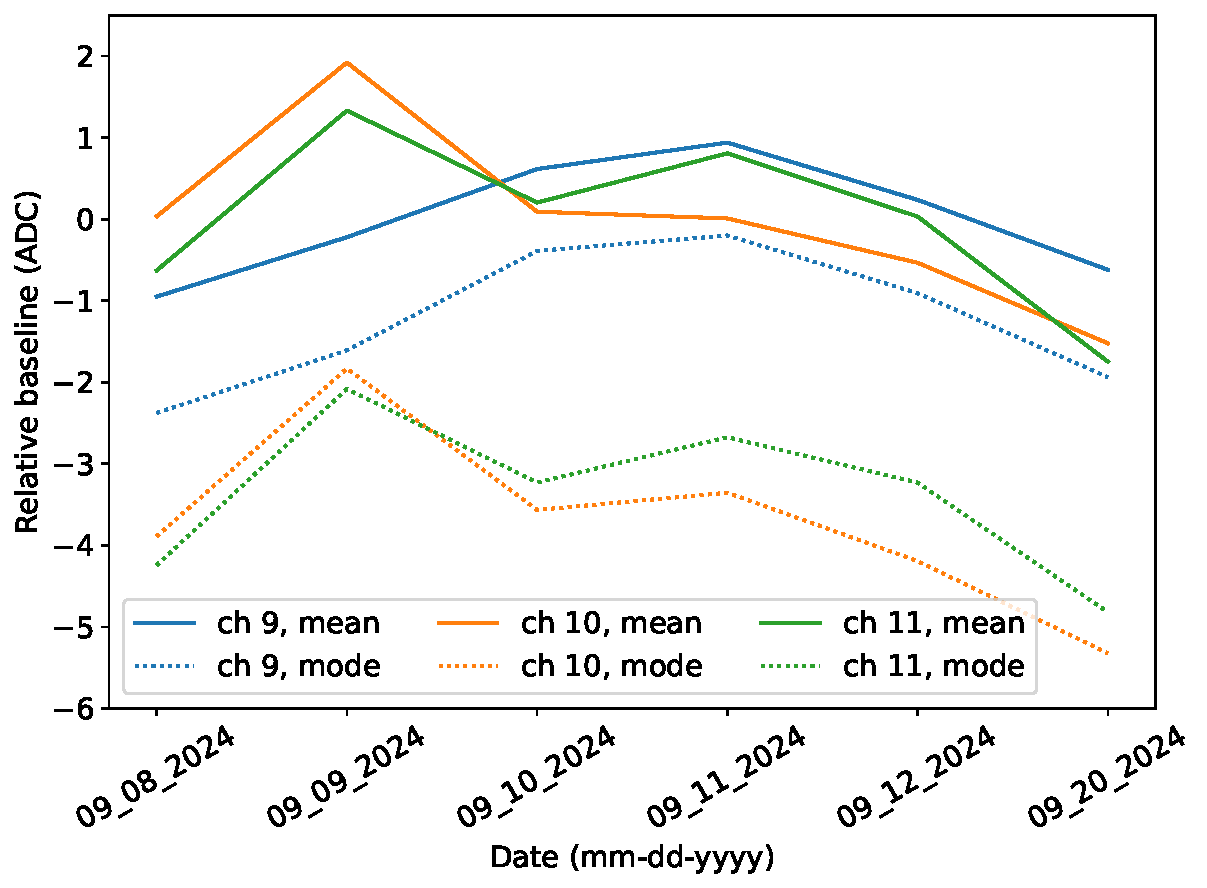
\includegraphics[width=0.477\textwidth]{images/baselines_rel2.pdf}
			\caption{.}
			\label{fig:baselines}
			\end{center}
	\end{figure}
	
	Plotting the 
	
	\begin{figure}[!h]
		\begin{center}
			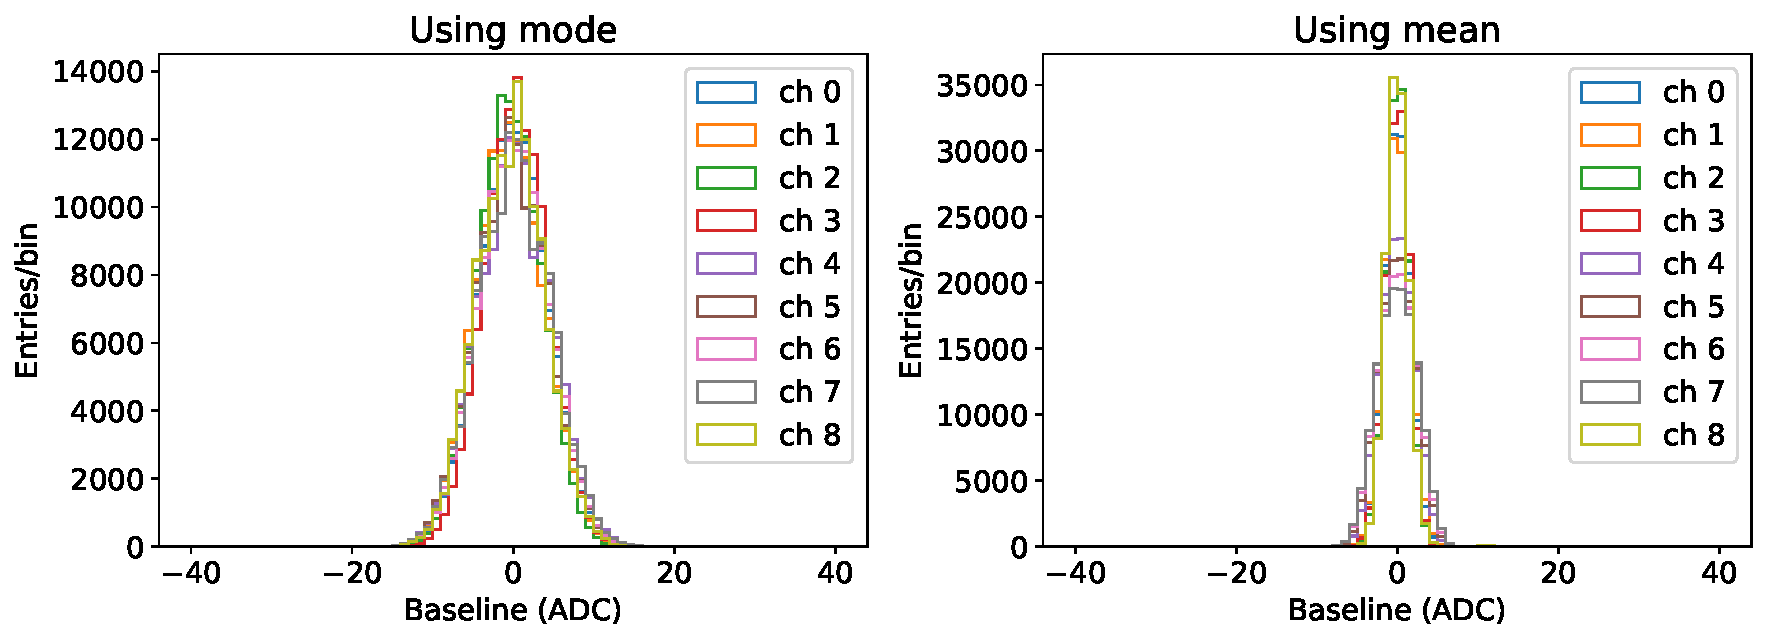
\includegraphics[width=\textwidth]{images/baselines_rel1_norm_ch.pdf}
			\caption{.}
			\label{fig:baselines2}
		\end{center}
	\end{figure}

	\begin{figure}[!h]
		\begin{center}
			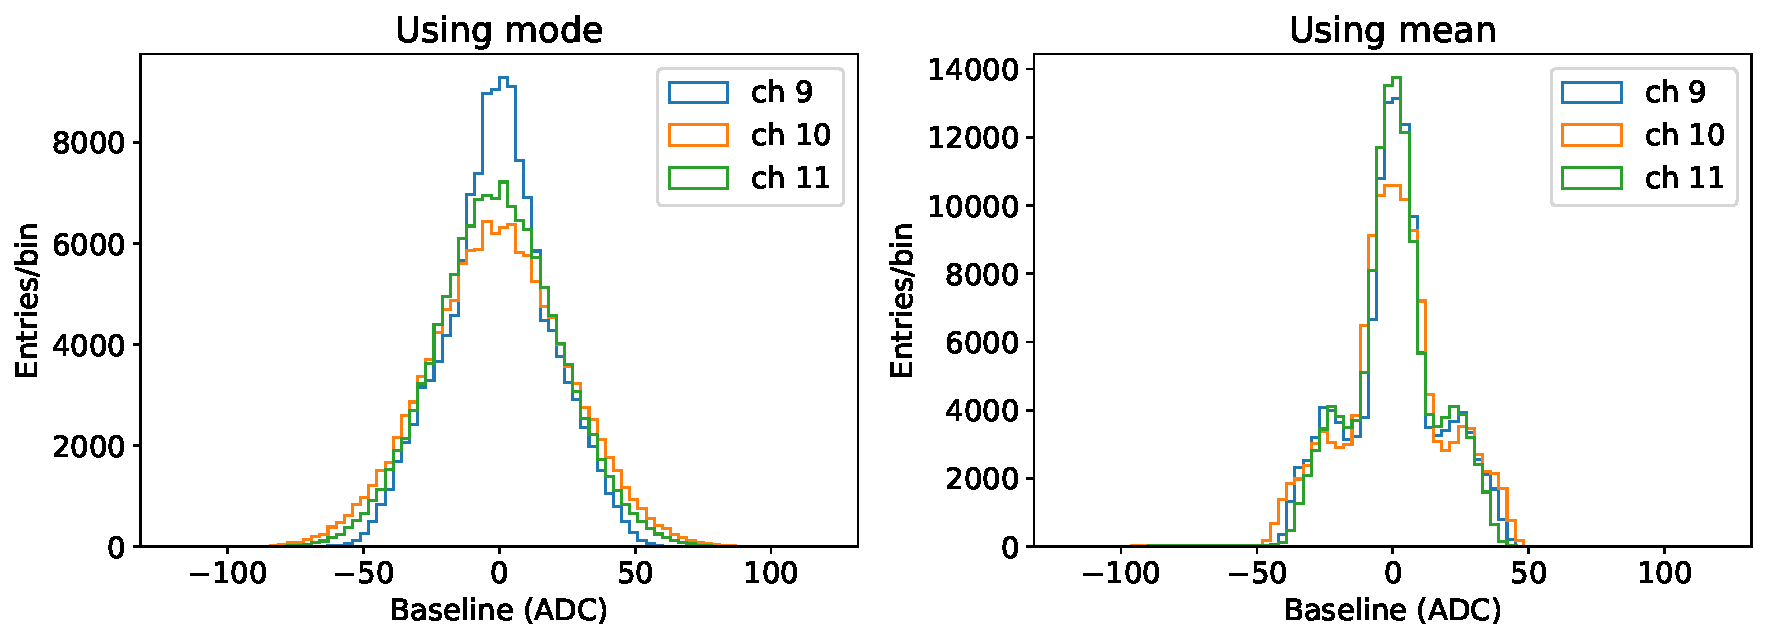
\includegraphics[width=\textwidth]{images/baselines_rel1_trigg_ch.pdf}
			\caption{.}
			\label{fig:baselines3}
		\end{center}
	\end{figure}	
	
	
	
\end{document}